% !TEX TS-program = XeLaTeX
% use the following command:
% all document files must be coded in UTF-8
\documentclass[english]{textolivre}
% build HTML with: make4ht -e build.lua -c textolivre.cfg -x -u article "fn-in,svg,pic-align"

\journalname{Texto Livre}
\thevolume{16}
%\thenumber{1} % old template
\theyear{2023}
\receiveddate{\DTMdisplaydate{2022}{10}{11}{-1}} % YYYY MM DD
\accepteddate{\DTMdisplaydate{2022}{11}{21}{-1}}
\publisheddate{\DTMdisplaydate{2023}{1}{2}{-1}}
\corrauthor{Xiaotong Yu}
\articledoi{10.1590/1983-3652.2023.41469}
%\articleid{NNNN} % if the article ID is not the last 5 numbers of its DOI, provide it using \articleid{} commmand 
% list of available sesscions in the journal: articles, dossier, reports, essays, reviews, interviews, editorial
\articlesessionname{articles}
\runningauthor{Yu et al.} 
%\editorname{Leonardo Araújo} % old template
\sectioneditorname{Daniervelin Pereira}
\layouteditorname{Leonado Araújo}

\title{Are educational robots any good for communicative English learning for primary school students?}
\othertitle{Os robôs educacionais são bons para o aprendizado comunicativo de inglês para alunos do ensino fundamental?}
% if there is a third language title, add here:
%\othertitle{Artikelvorlage zur Einreichung beim Texto Livre Journal}

\author[1]{Xiaotong Yu~\orcid{0000-0001-6161-2498}\thanks{Email: \href{mailto:xiaotong.yu01@estudiante.uam.es}{xiaotong.yu01@estudiante.uam.es}}}
\author[1]{Maria Angeles Gutierrez Garcia~\orcid{0000-0001-7376-6064}\thanks{Email: \href{mailto:nines.gutierrez@uam.es}{nines.gutierrez@uam.es}}}
\author[2]{Roberto Soto-Varela~\orcid{0000-0003-2105-5580}\thanks{Email: \href{mailto:roberto.soto@uva.es}{roberto.soto@uva.es}}}
\affil[1]{Autonomous University of Madrid, Department of Pedagogy, Spain.}
\affil[2]{University of Valladolid, Faculty of Education of Segovia, Spain.}

\addbibresource{article.bib}
% use biber instead of bibtex
% $ biber article

% used to create dummy text for the template file
\definecolor{dark-gray}{gray}{0.35} % color used to display dummy texts
\usepackage{lipsum}
\SetLipsumParListSurrounders{\colorlet{oldcolor}{.}\color{dark-gray}}{\color{oldcolor}}

% used here only to provide the XeLaTeX and BibTeX logos
\usepackage{hologo}

% if you use multirows in a table, include the multirow package
\usepackage{multirow}

% provides sidewaysfigure environment
\usepackage{rotating}

% CUSTOM EPIGRAPH - BEGIN 
%%% https://tex.stackexchange.com/questions/193178/specific-epigraph-style
\usepackage{epigraph}
\renewcommand\textflush{flushright}
\makeatletter
\newlength\epitextskip
\pretocmd{\@epitext}{\em}{}{}
\apptocmd{\@epitext}{\em}{}{}
\patchcmd{\epigraph}{\@epitext{#1}\\}{\@epitext{#1}\\[\epitextskip]}{}{}
\makeatother
\setlength\epigraphrule{0pt}
\setlength\epitextskip{0.5ex}
\setlength\epigraphwidth{.7\textwidth}
% CUSTOM EPIGRAPH - END

% LANGUAGE - BEGIN
% ARABIC
% for languages that use special fonts, you must provide the typeface that will be used
% \setotherlanguage{arabic}
% \newfontfamily\arabicfont[Script=Arabic]{Amiri}
% \newfontfamily\arabicfontsf[Script=Arabic]{Amiri}
% \newfontfamily\arabicfonttt[Script=Arabic]{Amiri}
%
% in the article, to add arabic text use: \textlang{arabic}{ ... }
%
% RUSSIAN
% for russian text we also need to define fonts with support for Cyrillic script
% \usepackage{fontspec}
% \setotherlanguage{russian}
% \newfontfamily\cyrillicfont{Times New Roman}
% \newfontfamily\cyrillicfontsf{Times New Roman}[Script=Cyrillic]
% \newfontfamily\cyrillicfonttt{Times New Roman}[Script=Cyrillic]
%
% in the text use \begin{russian} ... \end{russian}
% LANGUAGE - END

% EMOJIS - BEGIN
% to use emoticons in your manuscript
% https://stackoverflow.com/questions/190145/how-to-insert-emoticons-in-latex/57076064
% using font Symbola, which has full support
% the font may be downloaded at:
% https://dn-works.com/ufas/
% add to preamble:
% \newfontfamily\Symbola{Symbola}
% in the text use:
% {\Symbola }
% EMOJIS - END

% LABEL REFERENCE TO DESCRIPTIVE LIST - BEGIN
% reference itens in a descriptive list using their labels instead of numbers
% insert the code below in the preambule:
%\makeatletter
%\let\orgdescriptionlabel\descriptionlabel
%\renewcommand*{\descriptionlabel}[1]{%
%  \let\orglabel\label
%  \let\label\@gobble
%  \phantomsection
%  \edef\@currentlabel{#1\unskip}%
%  \let\label\orglabel
%  \orgdescriptionlabel{#1}%
%}
%\makeatother
%
% in your document, use as illustraded here:
%\begin{description}
%  \item[first\label{itm1}] this is only an example;
%  % ...  add more items
%\end{description}
% LABEL REFERENCE TO DESCRIPTIVE LIST - END


% add line numbers for submission
%\usepackage{lineno}
%\linenumbers

\begin{document}
\maketitle

\begin{polyabstract}
\begin{abstract}
This paper presents a pilot study that focuses on the exploratory and rapid prototyping within the human-in-the-loop control of a self-constructed and developed educational robot in assisting communicative English learning in primary Education in Madrid, Spain. The study sample was composed of 37 3rd graders that attended four English learning program sessions in November 2021, in which robot integration plays a leading role as learning material. To achieve the above, an easy-to-build, programmed and economical LEGO Education Mindstorms EV3 package was optioned. Pre-and-post questionnaires, classroom observations, and an evaluation sheet that measures self-evaluation, peer evaluation, and teacher evaluation were applied. The result reveals students’ perception of the pioneering robot and although preliminary, presents validation of the technology for English class assistance. Another finding suggests that students’ stress generated from communication in English among peers was reduced with the companion of the robot. Due to the nature of a pilot study, both the number of sessions and the sample size are limited to determine if the robot is helpful in students’ vocabulary acquisition in the long run. Further study is to be conducted with the pioneer model to teach vocabularies of different categories for a longer period. The findings of this pilot study will serve as a reference in the attempt to develop and reproduce promising robots to assist English teaching and learning that are accessible to public schools.

\keywords{Robot-assisted English learning \sep Communicative English learning \sep Exploratory prototyping \sep Rapid prototyping}
\end{abstract}

\begin{portuguese}
\begin{abstract}
Este artigo apresenta um estudo piloto que se concentra na prototipagem exploratória e rápida dentro do controle humano no circuito de um robô educacional autoconstruído e desenvolvido para auxiliar o aprendizado comunicativo de inglês no ensino fundamental em Madri, Espanha. A amostra do estudo foi de 37 alunos da 3ª série que participaram de quatro sessões de um programa de aprendizado de inglês em novembro de 2021, no qual a integração de robôs desempenha um papel de destaque como material de aprendizagem. Para alcançar o acima, foi escolhido um pacote LEGO Education Mindstorms EV3 fácil de construir, programado e econômico. Foram aplicados questionários pré e pós-observações em sala de aula e uma ficha de avaliação que mede a autoavaliação, a avaliação dos pares e a avaliação do professor. O resultado revela a percepção dos alunos sobre o robô pioneiro e, embora preliminar, apresenta validação da tecnologia para auxílio às aulas de inglês. Outro achado sugere que o estresse dos alunos gerado pela comunicação em inglês entre os pares foi reduzido com o acompanhamento do robô. Devido à natureza de um estudo piloto, tanto o número de sessões quanto o tamanho da amostra são limitados para determinar se o robô é útil na aquisição de vocabulário dos alunos a longo prazo. Mais estudos devem ser realizados com o modelo pioneiro para ensinar vocabulários de diferentes categorias por um período mais longo. Os resultados deste estudo piloto servirão como referência na tentativa de desenvolver e reproduzir robôs promissores para auxiliar o ensino e aprendizagem de inglês que sejam acessíveis às escolas públicas.

\keywords{Aprendizagem de inglês assistida por robô \sep Aprendizagem comunicativa de inglês \sep Prototipagem exploratória \sep Prototipagem rápida}
\end{abstract}
\end{portuguese}
% if there is another abstract, insert it here using the same scheme
\end{polyabstract}

\section{Introduction}\label{sec-intro}
\textcite{eaton_global_2010} emphasizes on the aim of language education in the 21st century being communicative-oriented and practical as in connecting people worldwide, instead of the way of learning that features drill and rote.  She further advocates on the usage of technologies to achieve the above as it breaks down geographical and physical barriers for students to realize cross-cultural communication with the target language (L2) in an authentic setting. To achieve this goal, English teaching staff are obligated to identify current challenges in students’ learning process and update themselves in altering teaching methods and techniques as well as the dominance of technology in order to promote the efficiency in their work \cite{kocaman_factors_2017}.

\posscite{kocaman_factors_2017} survey finds that the major obstacles impeding Spanish students from becoming consummate English speakers are firstly linguistically related as in weakness of vocabulary, its pronunciation and therefore a hampered speaking skill, followed by instructional issues due to the need of modification and update in teaching methods and materials adapted. Thirdly, students’ emotional factors play an important role in their English acquisition. According to \posscite{krashen_principles_1982} affective filter hypothesis, the relative success of second language learning is influenced by a learner's attitudes, also referred to as the affective variables or attitudinal factors including motivation, self-confidence, and anxiety. Negative emotions, precisely, including lack of desire, low self-esteem, as well as learning anxiety, the attribute to be discussed in this paper, impede and block language input to be delivered to language acquisition devices depending on the degree – the strength of the affective filter – of these emotions. With regard to the subject at hand, he further argues that the relationship between attitudinal factors such as anxiety and second language acquisition is stronger when students have practiced the target language in comprehensible “acquisition-rich” situations and are tested with the communicative type of tests. Subsequent research in this line have offered evidence, for instance, anxiety generated from low grades and comments from teachers have negatively affected students’ performance, self-confidence, and motivation toward foreign language learning \cite{chen_relationship_2004, dewaele_does_2018}. Finally, the insufficiency of aid from the teaching practitioners and parents and resources that foster practicing and self-teaching also contribute to the current situation of students’ learning outcome.

In reaction to elevate the efficiency of English teaching, teachers and instructors have been adapting themselves to the use of technology ever since the introduction of first-generation computers to education, as well as their revised iterations, especially now when an enormous advancement in technology has been made with Artificial Intelligence (AI) being implemented to assist foreign language learning \cite{tahiru_ai_2021}. Within the domain of English teaching as a second language precisely, it has been suggested as a helpful tool in providing organized support in assisting English writing \cite{gayed_exploring_2022}. the technology of AI has also been applied to develop autonomous interactive social robots which are later implemented as assistants in language teaching and learning. 

\subsection{Related work}\label{sec-normas}
Robot-assisted language learning (RALL) has become a widely explored field and has a history of nearly two decades since the initial field trial designed and conducted by \textcite{kanda_interactive_2004} to determine whether the English-speaking social robot Robovie has a positive impact on Japanese students’ English speaking competency. \textcite{gutierrez_garcia_smart_2017} suggested that interacting with objects such as smart toys and robots is beneficial for young children in developing a variety of cognitive, linguistic and communicative abilities. Until 2019, over 15 research studies have been conducted with the Nao robot, making it a popular humanoid applied in the industry. Robots with other functional diversities such as Dragonbot occupies the second place and makes zoomorphic, animal-like attributes another possible attempt in RALL \cite{van_den_berghe_social_2019, randall_survey_2020} These social robots are considered to be more “helpful, credible, informative and, enjoyable to interact with”, therefore provides an enjoyable learning environment \cite[p. 260]{van_den_berghe_social_2019}. Compared with the interaction with human instructors in traditional language classrooms, children are more willing to communicate with robotic agents, especially those who are particularly shy and unconfident \cite{wu_instructional_2015}.

Regarding the learning outcome, \textcite{lee_cognitive_2010} addressed the value of Mero and Engle’s efficiency (two self-developed semi-humanoid and pet robots) in improving students’ English-speaking competence; however, no significant listening ability enhancement was shown. A similar study conducted in Taiwan, China found out from both quantitative and qualitative data analysis that, with the assistance of a self-developed robot, students demonstrated noticeable enhancement in motivation and learning outcome \cite{wu_instructional_2015}.

Potential as they are, developing a pioneer robot for language class is usually time-consuming conversely, and requires a professionally technical group and sufficient funds to back it up, yet the fruit is not ready for large-scale implementation. In the most updated survey, researchers find out that, due to the limitation of current technology, even the Nao robot which is seen as the most potential in its category fails to recognize children’s utterances. Hence, robots still need a certain medium like a tablet to communicate with its users and despite the effort in developing the robotic agent and the teaching materials, the novelty effect still deeply concerns researchers and is seen as a tough rival \cite{van_den_berghe_social_2019}.

As discussed above, developing a pioneering robot requires a significant investment of both time and money, to speed up the producing process with a lower the budget, \textcite{zamfirescu-pereira_fake_2021} advocate exploratory prototyping including physical prototypes, video prototypes, and virtual simulations which demands researchers to diversify and maximize the design alternatives and rapidly prototype within them, challenging the options toward materials, users, and settings. By doing so, researchers can select the optimal model between divergent ideations. Once the selection is narrowed and shortlisted, actual interactions can be carried out with users in specified scenarios to try out the functionalities of the robot and make improvements if needed \cite{zamfirescu-pereira_fake_2021}.

During the rapid prototype process, students as users are seen as indispensable to be involved in the RALL research. \textcite{reich-stiebert_exploring_2020} stressed that after involving users in generating design decisions of usable products, tools, systems, interfaces, or software programs, their attitudes about the design object are more optimistic and are more willing to use it afterward. RALL research aims to produce reliable robotic agents to enhance students’ foreign language learning and increase the quality and diversity of their class activities, therefore, students´ positive attitude toward robots is a desired side effect to obtain.

\subsection{Research questions}\label{sec-conduta}
This pilot study focuses on the exploratory and rapid prototyping within the human-in-the-loop control of a self-constructed and developed educational robot in assisting communicative English learning in primary education. Students were surveyed about their motivations in various aspects towards English learning with and without the robot-assisted condition. The study aimed to answer the following research questions:

\begin{enumerate}
    \item Do students like the pioneering robot?
    \item Does the robot fulfill its purpose in assisting communicative English learning in class?
    \item Do students enjoy the learning process in the presence of our pioneering robot?
    \item Does provided enjoyment by the robot boost target language acquisition and how? 
\end{enumerate}

\section{Research design}\label{sec-fmt-manuscrito}

\subsection{Overview of the RALL system }
As the possibility of employing humanoid robots in language teaching has been explored at a large scale, our initiative is to add to the diversity of the appearance of robotic agents and maintaining the learners intrigued and learn English in a productive way in spite of the novelty effect. We chose the Lego Mindstorms Education EV3 kit which contains one programmable unit with an LCD screen, three motors, 4 kinds of sensors, and numerous buildable bricks. During the robot development process, we constructed a “Gyro Boy” and a “Puppy” according to the “core set” model instruction within the support application also provided by LEGO, however, these two models either require a stability configuration before usage or show difficulty in following indicator signals to execute move forward and turn commands.


\subsection{Development of the program}\label{sec-formato}
The Lego Mindstorms Education EV3 kit is widely used in children's programming classes for its simplicity. Compared to other robots used in RALL research, this one does not require professionals as technical support to finish its programming. That is to say, this kit is more accessible for teachers and researchers who have little knowledge and experience in programming and less budget to write codes for a specific language class. The programmable unit supports C, C++, JAVA, and Python if a more complicated task is to be performed. However, as an alternative, one can also start with the EV3 Classroom application that runs on visual LEGO language which is similar to Scratch.

To make the robot interactive, it should be able to follow and execute instructions delivered by the students. And to avoid the users from getting bored with mechanical responses, the robot needs to be equipped with a few reciprocal responses to encourage further interaction, even better, to surprise the users. Based on these guidelines, we programmed the robot as follows (\Cref{fig01}, \Cref{fig02}):

\begin{figure}[h!]
\centering
\begin{minipage}{.5\textwidth}
 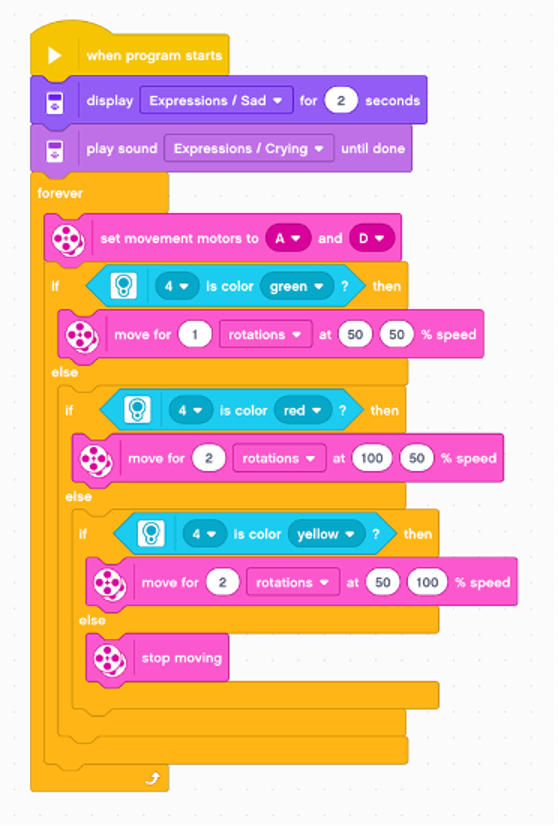
\includegraphics[width=\textwidth]{Fig1.png}
 \caption{Movement unit.}
 \label{fig01}
 \source{Own elaboration.}
\end{minipage}
\end{figure}

\begin{figure}[h!]
\centering
\begin{minipage}{.85\textwidth}
 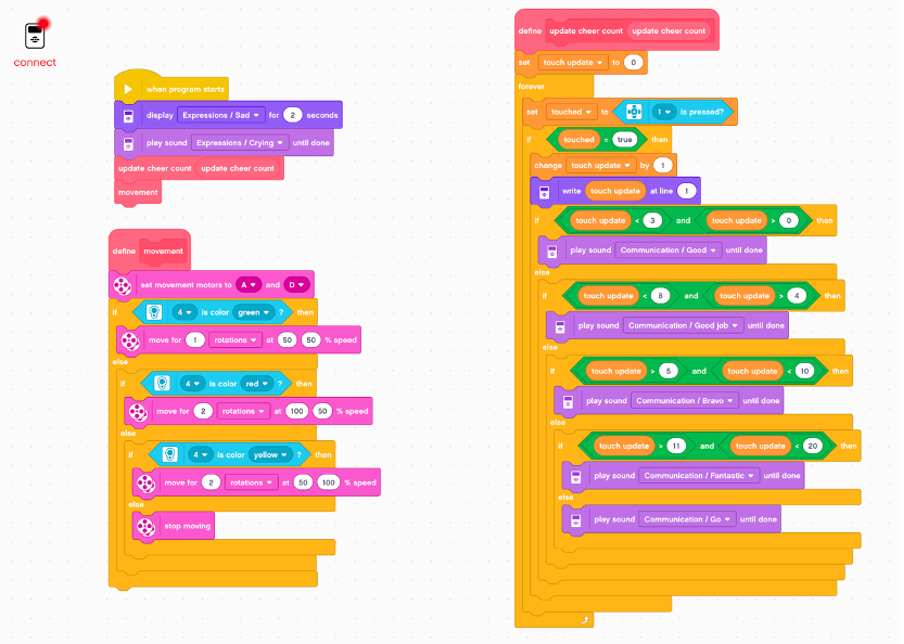
\includegraphics[width=\textwidth]{Fig2.png}
 \caption{Cheer unit.}
 \label{fig02}
 \source{Own elaboration.}
\end{minipage}
\end{figure}

Words restored in the library of the programmable unit are limited, yet it can still pronounce “good”, “go”, “good job”, “bravo”,and “fantastic”. The cheering words are triggered by the number of touches on the touch sensor. The revolutionary character of this program lies in the cheer unit, where a higher level of cheering is triggered by the accumulation of numbers of previous interactions while children are untold of this secret. Teachers and researchers can modify the number of interactions required to unblock the next level of verbal encouragement, also they can change the responses to other ones restored in the library.

Another advantage of these codes is that with this universal template, teachers are able to arrange class activities for the students to practice vocabularies and expressions of different categories (public establishments, professions, animals, transportation, etc.) and contexts.

\subsection{Development of the physical embodiment}\label{sec-modelo}
Inspired by \textcite{martin-ruiz_foundations_2015} smart toy design, the robot should look like a traditional toy with a considerate number of functional sensors detached within regular weight and size in order to attract children’s interest. From the broad library of core set models provided by LEGO in its EV3 Classroom application, both children and adults can follow the step-by-step instructions to construct solid robots. We chose the “Gyro Boy”, the “Puppy”, and a vehicle at the exploratory prototyping stage – named as “Driving Base”. “Gyro Boy”, as its name reflects, simulates a boy standing on his roller skates. It is color sensitive and can balance itself to move around. “Puppy” is inspired by a docile dog model; it can be fed and pet and responds to its owner with surprisingly charming non-verbal body language. As the movie Transformers is popular and influential worldwide, we also chose a simple vehicle embodiment and will later endow it with interactive attributes (\Cref{fig31}, \Cref{fig32}, \Cref{fig33}).

\begin{figure}[h!]
 \centering
 \begin{minipage}[t]{.30\textwidth}
 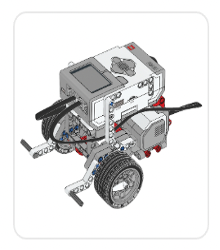
\includegraphics[width=\textwidth]{Fig31.png}
 \caption{Prototyped models - Vehicle.}
 \label{fig31}
 \source{Own elaboration.}
 \end{minipage}%
 \qquad
 \begin{minipage}[t]{0.30\textwidth}
 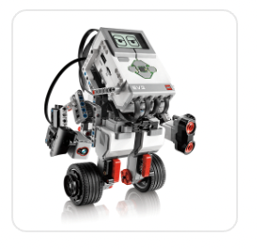
\includegraphics[width=\textwidth]{Fig32.png}
 \caption{Prototyped models - Gyro Boy.}
 \label{fig32}
 \source{Own elaboration.} 
 \end{minipage}%
  \qquad
 \begin{minipage}[t]{0.30\textwidth}
 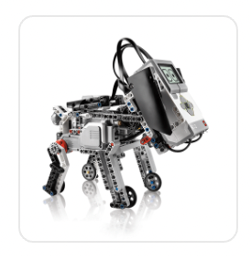
\includegraphics[width=\textwidth]{Fig33.png}
 \caption{Prototyped models - Puppy.}
 \label{fig33}
 \source{Own elaboration.} 
 \end{minipage}%
\end{figure}

During exploratory prototyping, attempts were made toward three appearance orientations, anthropometric, zoomorphic, as well as vehicle-like. The construction of these prototyped models “Gyro Boy”, “Puppy”, and “Driving Base” took up to 90-180 mins (90 steps with supporting base included), 125-250 mins (125 steps), and 45-90 mins (45 steps) respectively to be constructed by the researcher. As for horizontal prototyping, the “Driving Base” looks the least sophisticated while obtaining the best mobility among the three. In order to support its self-balancing functionality, one more component, the gyroscopic sensor, was attached to “Gyro Boy”. However, once departed from its initial set supporting base, “Gyro Boy” requires much time and effort to be configured and tends to fall and wiggle on the ground. To solve this problem, we attached it to its base. Although it managed to move it, the base impaired its smooth movement on the intervention panel, therefore this model was discarded. The same mobility issues were detected with “Puppy” as its hind legs were immobile, and the only two movement motors were set as its forelegs. Limited numbers of movement motors in the EV3 package failed to endow it with coordinate moment which led to the discarding of this model.

As for vertical prototyping, an additional pair of colored signal sticks shown in figure 6 was developed within two minutes. The colors “red”, “yellow”, and “green” were chosen as signals. The practice has proved that the color sensor is not sensitive enough to tell the difference between green and blue signals. The same robot behavior “go straight” was triggered by these colors. “White” also causes signal retrieving errors, this phenomenon is probably due to excessive reflection of red light as the signal approaches the sensor, hampering the accuracy of the color signal by considering its plastic texture.

\subsection{Scenario}\label{sec-organizacao}
Due to the simplicity of the pioneering robot, AI technologies are substituted at this stage of a pilot study with a narrative-based integrated episodic scenario (NIES) framework. NIES works by connecting the episodic scenarios with an overall cohesive narrative, resulting in a sequence of significant events that participants may empathize with and experience during the sessions. It gives participants a more holistic, ongoing, and focused contact experience with the research prototypes \cite{koay_prototyping_2016}.

In this case, on the day of the first session, a vehicle-looked robot is still in its newborn phase whose English level is similar to the learner’ is hidden inside the classroom, waiting for the students to find it. The reason why it is hiding is that it is very shy, as demonstrated in the figure below it has 5 facial expressions: lost, awake, smiling, joking, and satisfied.

Once a student finds the robot, he or she handles the robot for the researcher, and the robot will be turned on and let out a cry of agony because it is lost and confused about the situation. The rest of the class activities will take place in pairs, one student will guide the robot with colored signals and the other gives directions and descriptions of the surroundings. While all groups of students have gone through this process, they will exchange their roles and carry out the exercise once again. An example of the narrative used in some of the sessions is shown below:

\begin{quote}
    Today I [the researcher] am here in your English class because a little buddy that I know of is also in urgent need of your English lessons. It is very shy, so it has hidden somewhere in the classroom for you to find it and give it a warm welcome.
    
    At this moment it is still a baby, however, it grows up faster than you guys do. Now as you can see that it is crying because it lives permanently in that panel (the map) behind you. As perspicacious as you are, can you tell me what language people speak in its world?  English, right. As a baby and all by itself, it cannot read a single word and it is lost. Would you help it and show it around?
    
    It has grown a little older throughout the last week and it has learned a new human gesture – high-five. From now on, each time you take him to a new place, you can high-five it.
\end{quote}

\subsection{Experimental setup}\label{sec-organizacao-latex}
The target words are chosen from a worksheet on directions and the traffic and was adapted for students from 3rd to 5th graders. The theme is asking and giving directions and it focuses on vocabulary building and speaking. The objective of the learning sessions is to teach the students how to ask for and indicate directions using target vocabulary and expressions including prepositions and names of the different establishments. Students work in pairs to practice with the robot indicating where the robot stops, and complete the CARD B (\Cref{fig04}, \Cref{fig05}) earlier distributed to them with the names of the corresponding establishment once at a time.

\begin{figure}[htbp]
\centering
\begin{minipage}{.85\textwidth}
 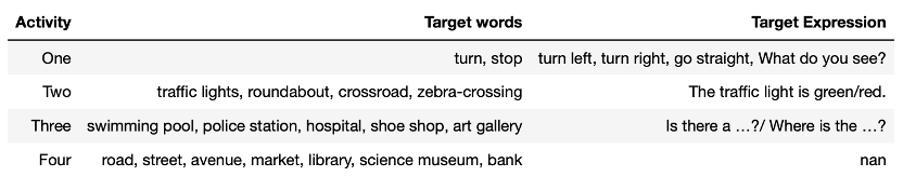
\includegraphics[width=\textwidth]{Fig4.png}
 \caption{Session plans.}
 \label{fig04}
 \source{Own elaboration.}
\end{minipage}
\end{figure}

\begin{figure}[htbp]
\centering
\begin{minipage}{.85\textwidth}
 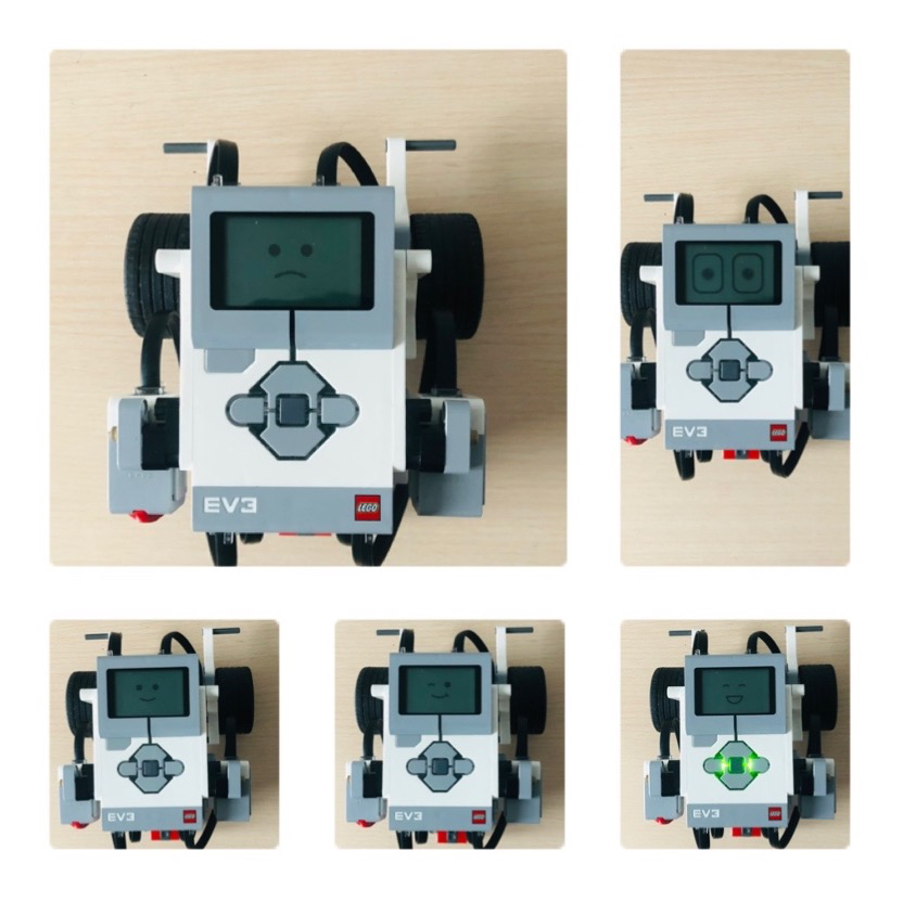
\includegraphics[width=\textwidth]{Fig5.png}
 \caption{Display of the prototyped model.}
 \label{fig05}
 \source{Own elaboration.}
\end{minipage}
\end{figure}

It moves steadily following three colored signals. The green signal drives it forward, while the students approach the “right hand” of the robot with the indicated signal stick, the color sensor reads the signal, and the wheels turn two rounds moving the robot straight ahead. Similarly, when approached with the yellow and red signals, the robot turns left and right respectively. For the first week of the training, only the movement part of the program will be activated. As the students gradually become consummate robot drivers, and they are taught vocabularies of different establishments by this time, they are allowed to high-five the left hand of the robot, where a touch sensor is located. To respond to this interaction, the robot pronounces “good”.  As the times of high-fives are multiplied to a certain number such as 3, 5, 8, and 11, the confused baby robot gets more oriented and pleased and it demonstrates how it feels with a corresponding facial expression and calls out “go”, “good job”, “bravo”, and finally “fantastic”.

Among the various instructional roles that a robot can adapt to, we define the role of the robot as a peer for two reasons. First, children tend to treat a robot as a peers in long-term interactions \cite{van_den_berghe_social_2019} and the current technology of automatic speech recognition (ASR) often fails when it comes to second language learners, especially when the users are children, because not only are there mispronunciation, misplaced lexical and grammar errors, but the structure the sentence could be completely disordered \cite{khalifa_joining--type_2016}, therefore hinders it from being class instructors (\Cref{fig06}).

\begin{figure}[htbp]
\centering
\begin{minipage}{.85\textwidth}
 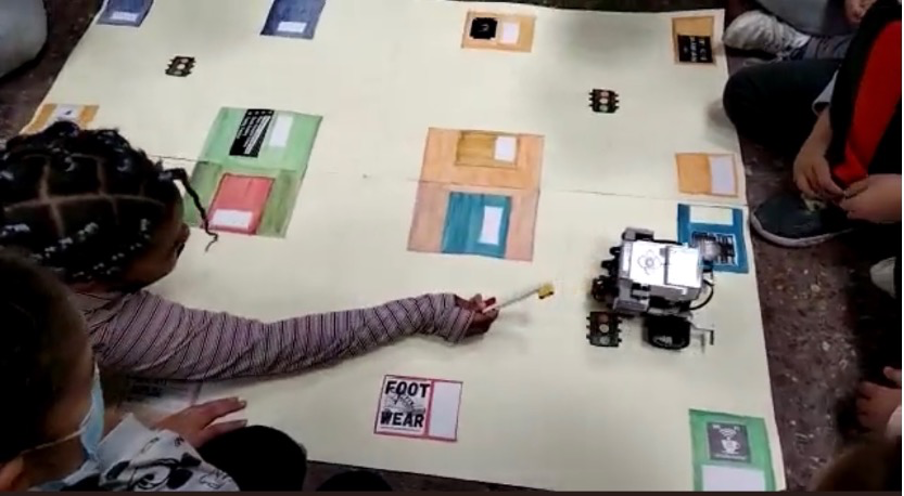
\includegraphics[width=\textwidth]{Fig6.png}
 \caption{Students practicing vocabulary with the robot on the map.}
 \label{fig06}
 \source{Own elaboration.}
\end{minipage}
\end{figure}

\section{Materials and methods}\label{sec-titulo}
To evaluate the effectiveness of the pioneering robot as an assistant to conduct communicative related learning activities, an experiment was conducted to compare the robot-assisted learning of children with the traditional method of teaching using PowerPoint slides, pencil and paper for notetaking. Consent was previously sent to be signed by the director of the school.

\subsection{Participants}\label{sec-idioma}
The experiment took place in the public primary school CEIP Jesús Varela in Alcorcón, Madrid. A total of 37 third grade students were involved in the intervention, however, because of sick leaves, only 33 students with an average age of 8.44 years (SD=0.61, range 7-10 years) have participated in all four sessions and submitted their feedback properly. Among them, 20 are girls and 13 are boys. All participants were selected through convenience sampling due to the fact that the research was conducted during the Covid-19 pandemic outbreak and the probability of sharing the pioneering robot on a large scale is obstructed. The students are from two parallel classes A and B although taught by different teachers.

\subsection{Data}\label{sec-resumo}
Data to support this study were collected from three major sources. A pre- and post- questionnaire was elaborated by the researcher to obtain information on students age, gender, years of experience in English learning, self-identified motivation toward participating in class activities, in realizing conversation in English in pairs or among groups, interest in English learning, stress in conducting speaking activities in pairs or among groups, as well as the degree of enjoyment provided by this robot-assisted condition. The two questionnaires are distributed to the students at the beginning and the end of all sessions.

Meanwhile, an evaluation sheet including self-evaluation, peer evaluation, and evaluation of the teachers will also be delivered to the learners at the first sessions to document their learning outcomes. Recalled words of each didactic session will be documented by the students themselves at the self-evaluation column when a session is done. Peer evaluation can be carried out during each session as students swap their evaluation sheets with their partner to rate their teamwork performance, activity fulfillment and usage of vocabulary. Teacher’s evaluation on students’ performance and language acquisition is realized when both students in the same working group have finished their practice.

Finally, field notes and short video clips taken by the teachers at the school were applied to document the performance of the pioneering robot, the events celebrated, student’s personal reactions including body language and tones, their points of view and any unexpected issues. To obtain the whole picture and a comprehensive understanding of the cultural group and their community, chats with the teachers are also implemented to complement participant observation \cite{shin_review_2022}. 

\subsection{Methods}\label{sec-secoes}
A mixed method approach was applied to address this exploratory research and data analysis is performed respectively. The qualitative approach of classroom observation is used in the first place. Classroom observation is a methodology for comparing two instructional methods between two randomly assigned groups. This methodology is very useful for testing and determining which method works best \cite{vidhiasi_dhion_classroom_2018}. The uniqueness of classroom observation lies in that data is obtained through interactions with the students in a natural setting with, for example, casual conversation, similar to participant observation \cite{shin_review_2022}. Since there is limited knowledge in the effectiveness of educational robots in assisting foreign language classes, this study has used classroom observation to understand both the participants and the capacity and functionality of the pioneering robot. As intervention is completed, the quantitative study is conducted. Python that runs on a Jupyter notebook was chosen for the descriptive analysis and data visualization. The inferential analysis was conducted with SPSS where an independent t-test was administered to support the pre- and post-test study design. The t-test is suitable for this research as our sample size is below 30 (n1=17, n2=16) for the two parallel classes A and B respectively. By using the t-test, we assumed that the population is normally distributed and made sure that the sample observations are independent.

The inferential statistical procedure calculates the probability of rejecting the null hypothesis that two means are the same \cite{gerald_brief_2018}, leaving us the alternative hypotheses: H1: students’ interest in English learning is different between the two groups; H2: students’ motivation in participating class activities is different between the two groups; H3: students’ motivation in realizing speaking exercise within pairs or groups is different; H4: students’ stress in conducting speaking activities in pairs or among groups is different; and, finally, H5: students’ degree of enjoyment provided by this robot-assisted condition is different between the two groups.

Due to mutual agreement of the principle of fairness, all students involved in this study should have experienced the robot-assisted condition, the alternative hypotheses are assumed to be accepted as students from class A will have already been taught the target words and then conduct the experiment while class B experience the robot-assisted learning directly. 

\section{Results}\label{sec-format-simple}

\subsection{Classroom observation }
To address questions 1 and 2, the researcher observed that students of both genders haven shown eagerness in interacting with the robots. During all of the four sessions, students were allowed to take the liberty in choosing their workmates. At the first session, the researcher remained a complete observer during the group forming process and did not shift to the role of observer as participant until all students had sat in a circle with their partners around the interaction panel with the robot and colored signals located in the middle. When a group of students had finished their interaction, the researcher asked them to go back to their seats and notice the students waiting to participate. The ultimate number of students that the panel could cater was around 8 so that students could scatter and move at ease.

During the interaction, students have exhibited consistent interest and curiosity toward the robot, as they anticipated to take turns in the interaction and discussed among themself to decide the order to volunteer. Frequently asked questions were related to the model specifications and coding details of the robot, Moreover, at least one student from each class reported having the same or similar LEGO Education Robotics Package in their personal collection and had programmed it differently. The rest of the students have had Digi Craft class – robot programming class – throughout this academic year, therefore, all participants in this sample have had previous experience with robotics.

With programs restored in the programmable unit, the LEGO EV3 robot could run on six AA/LR 6 batteries with full autonomy without being recharged throughout a total of 8 forty-minute sessions. The robot was configured to a higher social level and students demonstrated more curiosity and marveled when responded by the robot as they high-fived it or received verbal encouragement from it. Although the yellow signal for left turning occasionally failed and the robot moved forward instead, both the red and green signals worked with accuracy. As the robot cannot move backward, students with extraverted personality were more likely to hand-correct the trajectory of the robot when the wheels pressed on a line were supposed to be a wall or other obstacles alike. Nevertheless, no one has taken the robot aside from the panel to play with it alone. Shyness among some girls was detected for fear of making a show of themselves. Once they were confused with the signals or the robot moved in a direction otherwise than what they had intended, they showed hesitation to continue with the next approach.

When directly asked the students if they like the pioneering robot over casual talks, students all declared their attitude positively. To better perceive their preference towards robots’ appearance, pictures taken by the teachers of students’ plasticine handcrafts on their ideal robots produced during the waiting period in session 2 were taken into consideration. As can be seen in the \Cref{fig07}, students’ creations have in common to be human-like which led to the assumption that humanoids or anthropomorphic robots are more appealing to students.

\begin{figure}[h!]
\centering
\begin{minipage}{.5\textwidth}
 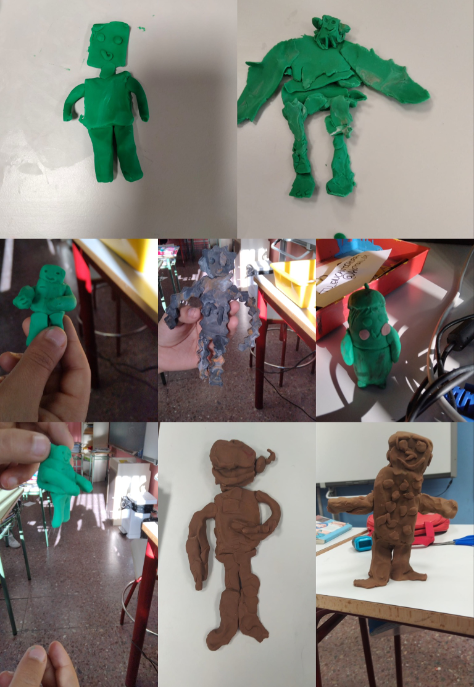
\includegraphics[width=\textwidth]{Fig7.png}
 \caption{Plasteline robot.}
 \label{fig07}
 \source{Own elaboration.}
\end{minipage}
\end{figure}

\subsection{Quantitative analysis}\label{sec-links}
In order to analyze the difference between the average number of words obtained by class A and B, an independent t-test was conducted in IBM SPSS Statistics 26. The data was drawn from students’ recalled words from the evaluation sheet with words obtained showed significant differences in session 2, tgl=31=34.68, p=0, and in session 3, tgl=32=4.78, p= 0, with the alpha value of .05. However, there were not significant differences in sessions 1 and 4 (\Cref{fig08}).

\begin{figure}[h!]
\centering
\begin{minipage}{.85\textwidth}
 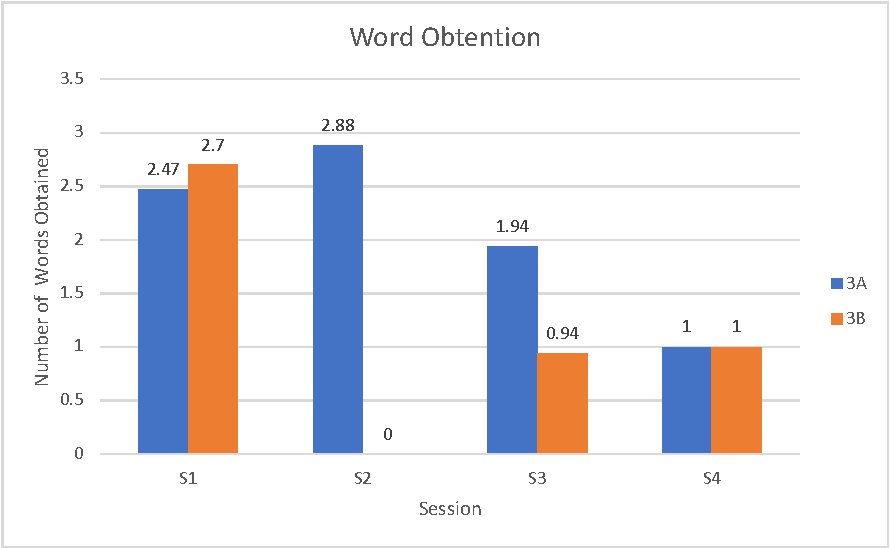
\includegraphics[width=\textwidth]{Fig8.pdf}
 \caption{Word Obtention.}
 \label{fig08}
 \source{Own elaboration.}
\end{minipage}
\end{figure}

The results clearly show that students in class A (blue column) recalled an average of 3.65 more words than in class B (orange column). Interestingly, however, students in class B ranked a higher score after the first session (average of 2.7) even though class A have been taught the target words beforehand. In addition, the sharp fall as shown in figure 8 of vocabulary acquisition in session 2 suggests an inconsistency in the learning and retention of the target words although followed by a gradual increase. Nevertheless, the lower word obtention rate of class B is not necessarily related to the ineffectiveness of RALL as students of class A have already studied the target words while they were waiting for the experiment.

Students in two classes expressed higher stress levels realizing speaking activities in English among peers (average of 4.35 for class A and average of 4 for class B) without a robot than in robot-assisted conditions (average of 1.41 and 1.82 respectively) $tgl=37=6.8, p=0$. Results on variables such as motivation are not statistically significant in the research. It can be argued that the questions surveyed in this aspect assessed in this pilot study were maybe too concrete and general to detect nuances for students at this age.

The students’ stress level when speaking English with their partners was lower in robot condition (average of 1.62) than in non-robot condition (average of 4.19) as shown in \Cref{fig09}.

\begin{figure}[h!]
\centering
\begin{minipage}{.85\textwidth}
 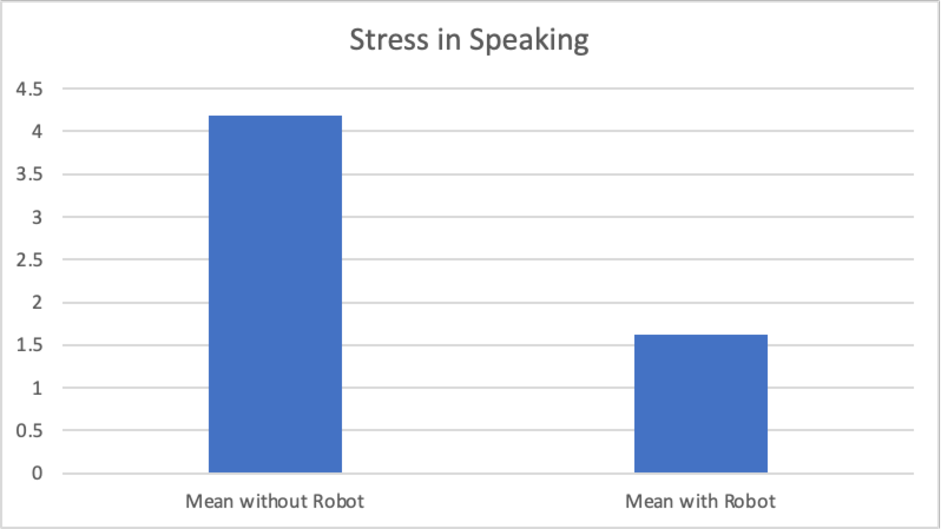
\includegraphics[width=\textwidth]{Fig9.pdf}
 \caption{Stress in Speaking.}
 \label{fig09}
 \source{Own elaboration.}
\end{minipage}
\end{figure}

\section{Discussion}\label{sec-outras-estr}
The main purpose of this study is to explore and rapidly prototype within the human-in-the-loop control of a self-constructed and developed educational robot in assisting communicative English learning in primary education. One interesting finding is that instead of a fully autonomous social robot, a relatively economical LEGO Mindstorm EV3 Package achieves the goal similarly. Moreover, the prototyped model does not require consistent modification and can be adapted as a universal model to the teaching of diverse categories and themes of vocabulary, such as fauna, flora, and professions.

Surprisingly, the novelty effect stressed in the literature \cite{diaz_building_2011,han_physical_2009,van_den_berghe_social_2019,yamamoto_trial_2006} was not detected in this study, a student’s study outcome of the experimental group increased after an abrupt drop. One possible explanation might relate to insufficient numbers of sessions for this phenomenon to manifest. Also, unlike what literature stressed that imaginable words are more easily remembered \cite{ellis_essentials_2019,lupyan_words_2015}, students in both classes demonstrated better recalling of abstract words and expressions such as “go straight”, “turn left/right”. This inconsistency may be due to frequent repetition as they were taught during the first session and were put into practice since then. Another possible explanation for this is that these words were the only ones with which students directly interact with the robot. 

The most important academic relevant finding was that students in the control group have obtained a larger amount of target words. This finding inevitably leads to the reflection of the research design as they were already taught and familiar with the target words while the experimental group carried out the learning directly in a robot-assisted condition. Finally, data suggested that the robot-assisted didactic session was pleasant and enjoyable and a significant reduction in stress suffered in the speaking activity occurred, which gave a chance to the practical appliance of primary school English teaching and learning.

Align with \textcite{han_physical_2009}, the result of this study suggested that robotic agents may create an enjoyable learning environment, and could help students to develop social and interpersonal skills \cite{diaz_building_2011,mubin_review_2013}.


\section{Conclusions}\label{sec-listas}
This study set out to determine the possible potential of a simplified model, instead of a fully functional AI integrated robot, in assisting primary school English teaching and learning in a public school in Spain. The experience with the pioneering robot helped us to obtain some initial answers to the questions raised in the research. As for the first research question whether the students like the pioneering robot, the answer is affirmative, as students have verbally expressed their fondness of the robot and their continuous interest and curiosity toward the robot has spoken for itself. The second aim of the research was to test the capability of the pioneering robot in assisting communicative English learning in class. The experiment confirmed that the functionality of the current prototype not only survived eight forty-minute sessions but is also user-friendly. Despite occasional failures and misbehave of the robot caused by inappropriate approach of the signal to the color sensor, students now and then lingered to ask questions and comment on the activity. No unexpected incident or major technical failure occurred during the process. Although affirmative answers and the learning outcome is obtained for students of both classes, due to the limitations of this research, it still remains ambiguous whether the students enjoy the learning process in the presence of our pioneering robot and if the enjoyment provided by the robot can be regarded as a booster in foreign language acquisition.

Firstly, limited by the number of robots available and the size of the panel, the circle formed by students appeared to be crowded and during interaction, inevitable knee touches and altercation occurred which led the teacher to recall half of the students back to their seats to conduct other activities. Uncomfortable experience may have a negative effect on students’ perception on the RALL intervention. Secondly, the level of stress registered in this study is self-perceived as we had only formulated this variable as a possible factor that affects foreign language learning. In the next step, we consider including the Foreign Language Classroom Anxiety Scale (FLCAS) to obtain a relatively unbiased and objective perception toward students’ level of stress in L2 learning the next step, as research on a larger scale is conducted and with a fully functional AI implemented pioneering robot.

Furthermore, needless to say, our results are preliminary and await completion of the ongoing work, as well as subsequent replication with a larger sample. Respecting the school policy, all students went through the same robot-assisted process when this experiment was to be conducted, thus leaving us with no non-robot-assisted condition to compare the learning outcome with. By involving students from different institutions, we can both enlarge the study sample and obtain a proper control group. To avoid the aforementioned flaws that emerged in this pilot study, one insight this study provides for future research would be that different sets of targets words should be distributed to the experimental and the control group, for that only the number of words correctly recalled will be taken into account for data analysis, therefore, it is unnecessary for both groups to adapt to the identical target words. Also, it is recommended that the hours of exposure to robotic agents varies in different groups for the affirmation of reduction of novelty effect.

\section{Acknowledgements}\label{sec-figuras-tabelas}
The team would like to thank all staff who facilitated this research and students from public school Jesús Varela who took part in it.


\printbibliography\label{sec-bib}
% if the text is not in Portuguese, it might be necessary to use the code below instead to print the correct ABNT abbreviations [s.n.], [s.l.]
%\begin{portuguese}
%\printbibliography[title={Bibliography}]
%\end{portuguese}


%full list: conceptualization,datacuration,formalanalysis,funding,investigation,methodology,projadm,resources,software,supervision,validation,visualization,writing,review
\begin{contributors}[sec-contributors]
\authorcontribution{Xiaotong Yu}[conceptualization,datacuration,investigation,writing,review]
\authorcontribution{Maria Angeles Gutierrez Garcia}[methodology,projadm,resources,validation,writing,review]
\authorcontribution{Roberto Soto-Varela}[projadm,supervision,resources,writing,review]
\end{contributors}


\end{document}

